\documentclass[twocolumn, traditabstract]{aa}  

\usepackage{fixltx2e}
\usepackage[english]{babel}
\usepackage{graphicx,amsmath}
\usepackage{epstopdf}
\usepackage{epsf,color}
\usepackage[mathscr]{eucal}
\usepackage{amsmath}
\usepackage{amssymb,amsfonts}
\usepackage{natbib}
\usepackage{txfonts}
\usepackage{dsfont}
\definecolor{Mygreen}{rgb}{0.00, 0.72, 0.0}
\definecolor{Mypink}{rgb}{1.0, 0.0, 0.5}
\usepackage[breaklinks, citecolor=blue, linkcolor=Mygreen, urlcolor=Mypink, colorlinks=true, debug, baseurl=' ']{hyperref}
\usepackage{float}
\usepackage{color}
\usepackage{scrextend}
\usepackage{nccmath}
\usepackage{mathtools, cuted}
\usepackage{lscape}
%\usepackage{widetext}
\usepackage{flushend}
\usepackage[T1]{fontenc}
\usepackage{gensymb}
\usepackage{diagbox}



\newcommand{\nika}{{\it NIKA}}
\newcommand{\nikad}{{\it NIKA2}}
\newcommand{\Q}{$Q$}
\newcommand{\I}{$I$}
\newcommand{\U}{$U$}
\newcommand{\di}{$dI$}
\newcommand{\dq}{$dQ$}
\newcommand{\eps}{$\varepsilon$}
\newcommand{\epsCMB}{$\varepsilon_{CMB}$}
\newcommand{\epsDET}{$\varepsilon_{det}$}
\newcommand{\rf}{{\it RfdIdQ}}
\newcommand{\cf}{{\it Cf}}


\def\simlt{\lower.5ex\hbox{$\; \buildrel < \over \sim \;$}}
\def\simgt{\lower.5ex\hbox{$\; \buildrel > \over \sim \;$}}
\def\NIKA{\textit{NIKA}}

\bibpunct{(}{)}{;}{a}{}{,}
\bibliographystyle{aa}

\begin{document}
\title{KID systematics and CMB polarization blabla}
%\author{R.~Adam \inst{\ref{OCA},\ref{LPSC},\ref{CEFCA}}\thanks{Corresponding author: R\'emi Adam, \url{remi.adam@oca.eu}}
\and O.~Hahn\inst{\ref{OCA}}						%NCT
\and  F.~Ruppin \inst{\ref{LPSC}}
\and  P.~Ade \inst{\ref{Cardiff}}
\and  P.~Andr\'e \inst{\ref{CEA}}
\and M.~Arnaud\inst{\ref{CEA}}					%NCT
\and I.~Bartalucci\inst{\ref{CEA}}					%NCT
\and  A.~Beelen \inst{\ref{IAS}}
\and  A.~Beno\^it \inst{\ref{Neel}}
\and  A.~Bideaud \inst{\ref{Neel}}
\and  N.~Billot \inst{\ref{IRAME}}
\and  O.~Bourrion \inst{\ref{LPSC}}
\and  M.~Calvo \inst{\ref{Neel}}
\and  A.~Catalano \inst{\ref{LPSC}}
\and  G.~Coiffard \inst{\ref{IRAMF}}
\and  B.~Comis \inst{\ref{LPSC}}
\and  A.~D'Addabbo \inst{\ref{Neel},\ref{Roma}}
\and  F.-X.~D\'esert \inst{\ref{IPAG}}
\and  S.~Doyle \inst{\ref{Cardiff}}
\and C.~Ferrari\inst{\ref{OCA}}						%NCT
\and  J.~Goupy \inst{\ref{Neel}}
\and  C.~Kramer \inst{\ref{IRAME}}
\and  G.~Lagache \inst{\ref{LAM}}
\and  S.~Leclercq \inst{\ref{IRAMF}}
\and  J.-F.~Lestrade \inst{\ref{LERMA}}
\and  J.F.~Mac\'ias-P\'erez \inst{\ref{LPSC}}
\and G.~Martinez Aviles\inst{\ref{OCA}}				%NCT
\and D.~Martizzi\inst{\ref{Berkeley}}					%NCT
\and S.~Maurogordato\inst{\ref{OCA}}				%NCT
\and  P.~Mauskopf \inst{\ref{Cardiff},\ref{Arizona}}
\and  F.~Mayet \inst{\ref{LPSC}}
\and  A.~Monfardini \inst{\ref{Neel}}
\and  F.~Pajot \inst{\ref{IAS}}
\and  E.~Pascale \inst{\ref{Cardiff}}
\and  L.~Perotto \inst{\ref{LPSC}}
\and  G.~Pisano \inst{\ref{Cardiff}}
\and E.~Pointecouteau\inst{\ref{IRAP}, \ref{UniToulouse}}%NCT
\and  N.~Ponthieu \inst{\ref{IPAG}}
\and G.W.~Pratt\inst{\ref{CEA}}					%NCT
\and  V.~Rev\'eret \inst{\ref{CEA}}
\and M.~Ricci\inst{\ref{OCA}}						%NCT
\and  A.~Ritacco \inst{\ref{IRAME}}
\and  L.~Rodriguez \inst{\ref{CEA}}
\and  C.~Romero \inst{\ref{IRAMF}}
\and  H.~Roussel \inst{\ref{IAP}}
\and  K.~Schuster \inst{\ref{IRAMF}}
\and  A.~Sievers \inst{\ref{IRAME}}
\and  S.~Triqueneaux \inst{\ref{Neel}}
\and  C.~Tucker \inst{\ref{Cardiff}}
\and H.-Y.~Wu\inst{\ref{CalTech}}					%NCT
\and  R.~Zylka \inst{\ref{IRAMF}}}

\institute{
  Laboratoire Lagrange, Universit\'e C\^ote d'Azur, Observatoire de la C\^ote d'Azur, CNRS, Blvd de l'Observatoire, CS 34229, 06304 Nice cedex 4, France
  \label{OCA}
  \and
  Laboratoire de Physique Subatomique et de Cosmologie, Universit\'e Grenoble Alpes, CNRS/IN2P3, 53, avenue des Martyrs, Grenoble, France
  \label{LPSC}
    \and
  Centro de Estudios de F\'isica del Cosmos de Arag\'on (CEFCA), Plaza San Juan, 1, planta 2, E-44001, Teruel, Spain
  \label{CEFCA}
  \and
Institut de RadioAstronomie Millim\'etrique (IRAM), Grenoble, France
  \label{IRAMF}
\and
Laboratoire AIM, CEA/IRFU, CNRS/INSU, Universit\'e Paris Diderot, CEA-Saclay, 91191 Gif-Sur-Yvette, France 
  \label{CEA}
\and
Astronomy Instrumentation Group, University of Cardiff, UK
  \label{Cardiff}
\and
Institut d'Astrophysique Spatiale (IAS), CNRS and Universit\'e Paris Sud, Orsay, France
  \label{IAS}
\and
Institut N\'eel, CNRS and Universit\'e Grenoble Alpes, France
  \label{Neel}
\and
Institut de RadioAstronomie Millim\'etrique (IRAM), Granada, Spain
  \label{IRAME}
\and
Dipartimento di Fisica, Sapienza Universit\`a di Roma, Piazzale Aldo Moro 5, I-00185 Roma, Italy
  \label{Roma}
\and
Univ. Grenoble Alpes, CNRS, IPAG, F-38000 Grenoble, France 
  \label{IPAG}
    \and
Aix Marseille Universit\'e, CNRS, LAM (Laboratoire d'Astrophysique de Marseille) UMR 7326, 13388, Marseille, France
  \label{LAM}
\and
School of Earth and Space Exploration and Department of Physics, Arizona State University, Tempe, AZ 85287
  \label{Arizona}
\and
Universit\'e de Toulouse, UPS-OMP, Institut de Recherche en Astrophysique et Plan\'etologie (IRAP), Toulouse, France
  \label{IRAP}
\and
CNRS, IRAP, 9 Av. colonel Roche, BP 44346, F-31028 Toulouse cedex 4, France 
  \label{IRAP2}
\and
University College London, Department of Physics and Astronomy, Gower Street, London WC1E 6BT, UK
  \label{UCL}
\and 
Institut d'Astrophysique de Paris, Sorbonne Universit\'es, UPMC Univ. Paris 06, CNRS UMR 7095, 75014 Paris, France 
  \label{IAP}
\and 
LERMA, CNRS, Observatoire de Paris, 61 avenue de l'Observatoire, Paris, France
  \label{LERMA}
  \and  
Department of Astronomy, University of California, Berkeley, CA 94720-3411, USA
  \label{Berkeley}
    \and
Universit\'e de Toulouse, UPS-OMP, Institut de Recherche en Astrophysique et Plan\'etologie (IRAP), Toulouse, France
  \label{IRAP}
\and
CNRS, IRAP, 9 Av. colonel Roche, BP 44346, F-31028 Toulouse cedex 4, France 
  \label{UniToulouse}
  \and
California Institute of Technology, MC 367-17, Pasadena, CA 91125, USA.
  \label{CalTech}  
}


\date{Received \today \ / Accepted --}
	
\abstract{Here goes the abstract}
\titlerunning{KIDs systematics}
\authorrunning{TBD}
\keywords{Techniques: polarization -- KIDs --  individual: NIKA }
\tableofcontents
\maketitle

\section{Introduction}
\label{sec:introduction}

%Pour citer les papiers: \citep{planck2013mission} ou alors
%\citep{2010A&A...518L.100M,arzoumianian}.


%\begin{itemize}
%\item Why we want to measure CMB polarization B modes
%\item The need for matrices and the KID solution, quickly mention other
%  solutions and multiplexing
%\item Importance to master systematic effects (ref. to previous papers)
%\item KIDs are a new technology that has not yet reached a ``space proof''
%  maturity. In this paper, we address a few specific systematics to KIDs.
%\item Outline
%\end{itemize}

The measurement of CMB polarization, and especially the detection of $B$ modes, is
one of the major challenges in modern cosmology. In fact, a key motivation for
CMB polarization measurements is the theory of cosmic inflation. $B$ modes can be
generated by two mechanisms : gravitational lensing of $E$ modes
\citep{2013PhRvL.111n1301H}, or by gravitational waves produced during
inflation. The detection of primordial B modes would represent an indirect
detection of primordial gravitational waves, and as a result, establish the
theory of cosmic inflation.\\ In order to detect B modes, we need to study the
universe at high sensitivity. To do so, the development of
large detectors arrays is required.  The most used kind of detectors are
bolometers named Transition Edge Sensors (TES), but now their performances are
limited by the photon noise. It is possible to do medium-sized arrays of TES
detectors (1000 pixels), but developing larger arrays gets complicated for
technical and economical reasons. Other detectors used are Cold Electron
Bolometer (CEB) \citep{2007stt..conf...93K} and Superconducting Tunnel Junctions
(STJ) but they face difficulties in the fabrication process making them not
suitable for large arrays. Bolometers have enjoyed considerable technical
improvements but further array scaling is strongly limited by the multiplexing
factor of the readout electronics, consequently it was necessary to develop
detectors adapted to strong frequency domain multiplexing.\\ In this context, a
new kind of detectors was developed : the Kinetic Inductance Detectors (KIDs),
proposed by \citet{2003Natur.425..817D}. Since 2007, these detectors have been
developed for the construction of NIKA2 and its prototype NIKA (New IRAM Kids
Arrays), which is the first operational instrument using KIDs
\citep{2010A&A...521A..29M,2016JLTP..184..816C}. The main characteristic that
makes KIDs one of the best candidates to large size detector array is their
natural multiplexing capability. Indeed, the resonant frequencies of a resonator
can be easily controlled during the array design, and the sharpness of the
resonances allows many resonators to be placed into a limited band-width. Thus,
a large number of resonators, can be coupled to a single transmission line, each
one resonating at a different frequency $f_{0}^{i}$ \citep{2010A&A...521A..29M,
  Calvo2008}.\\ Together with high sensitivity, a strict control of systematic effects must be achieved. In fact, due to its faintness, The B-mode polarization can be easily degraded by various systematic
effects and it is important to remove these spurious contributions. Some of
these effects can be reduced in the design of the instruments while others have
to be simulated and corrected a posteriori. Numerous systematic effects arise
from optical and instrumental imperfections, temperature drifts of the optics
and detectors, contaminations by astrophysical foregrounds and te detector
non-linearity. These effects can be modelled and characterized by the spurious
signal $C_{l}$ they produce. For more details see \citep{2008PhRvD..77h3003S,
  quickpol} and references therein.\\ KIDs are a new technology that are now
routinely used in ground-based telescopes. However, in view of futur
uses above the atmosphere, we still have to demonstrate their
compatibility with a space mission (such as COrE \citep{2016arXiv160907263D}),
hence the need to master their sytematic effects. In this paper, we adress a few
specific systematics to KIDs. The paper is organized as follows:
Sect. \ref{sec2} presents a brief description of KIDs...

\section{Overview of KIDs}
\label{sec2}
\subsection{KID physics}

Kinetic inductance detectors are a novel superconducting detector technology that provides high sensitivity and ease of multiplexing. In this section we give a brief summary of the main features of KIDs.\\
KIDs are RLC superconducting resonators made from a thin metal film that react to an incoming radiation by changing their electromagnetic properties. In fact, when photons are absorbed by the superconducting film, they break Cooper pairs which increases the quasi-particles density and causes a change in the kinetic inductance $L_{k}$. This produces a shift, $\delta f_{0}$, of the resonant frequency of the KID \citep{2013A&A...551L..12C} that can be related to the absorbed optical power $\delta P_{opt}$. This relation is linear for small variations in $P_{opt}$ \citep{2010ApPhL..96z3511S}. The operating principle is represented in Fig.~\ref{resonance}.\\

\begin{figure}[h]
\center
	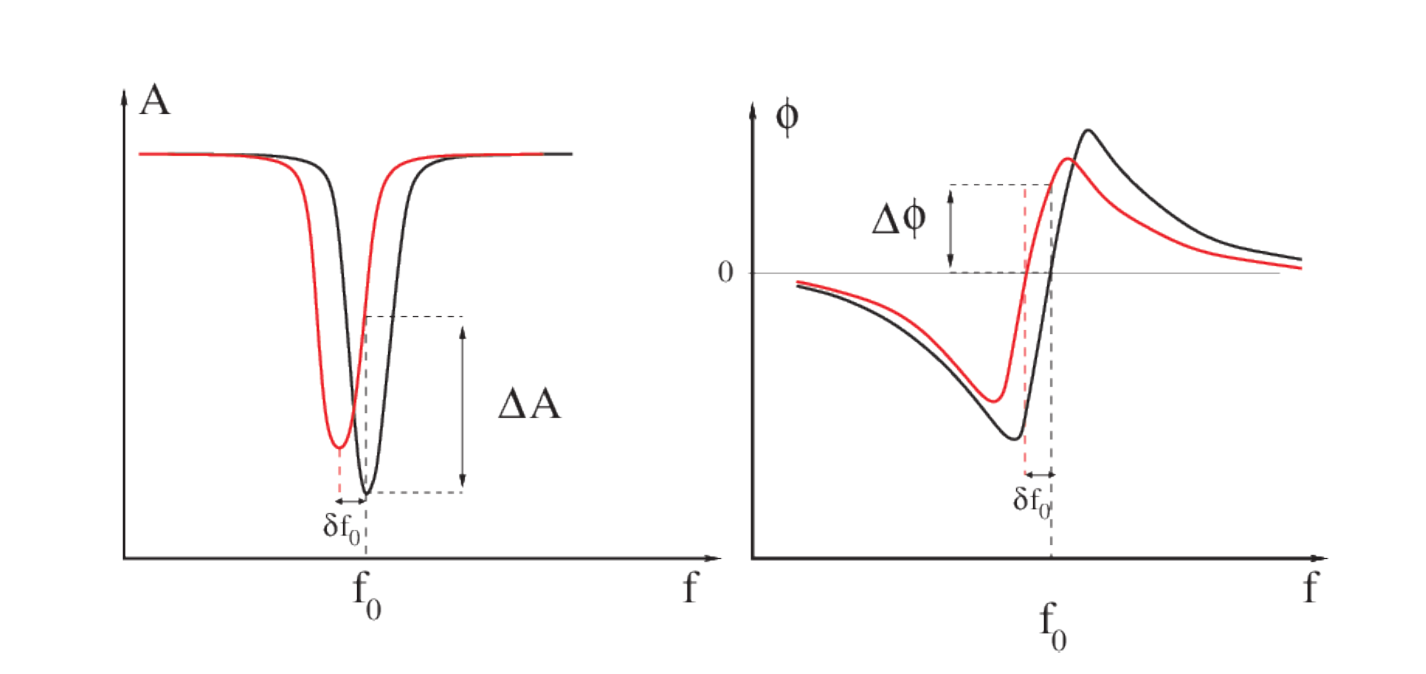
\includegraphics[scale=0.4]{Figures/resonance.png}
	\caption{Schematic representation of a KID resonance in amplitude (left) and phase (right), as a function of the excited tone injected in the feedline. The optical power absorbed by the detector is weak for black curves and increases for red curves. The absorption of a photon shifts the resonance frequency and this is directly proportional to the received power.}
	\label{resonance}
\end{figure}

The KID transfer function is given by :

\begin{equation}
S_{21}(f) = I +jQ .
\end{equation}

where \I\  and \Q\  give respectively the real (in phase) and imaginary (quadrature) of $S_{21}$.

\subsection{KID model}
A model of a KID transfer function has been proposed by \citet{2008ApPhL..93m4102G} :

\begin{equation}
S_{21} = \frac{2Z_{res}Z_{0}}{Z_{res}[2Z_{0} + j(X_{1}+X_{2})] + (Z_{0} +jX_{1})(Z_{0} +jX_{2})},
\end{equation}

with :

\begin{equation}
Z_{res} = \frac{Z_{0}Q_{e}}{2Q_{i}}[1 + 2jQ_{i}\frac{(f-f_{0})}{f_{0}}],
\end{equation}

where $X_{1}$, $X_{2}$, $Z_{0}$ are impedances, $Q_{i}$ is the intrinsic quality factor of the resonator and $Q_{e}$ is the external quality factor due to coupling with the measurement electronics. $f$ is the frequency of excitation of the detector, and $f_{0}$ is the resonant frequency. Throughout this paper, we shall assume typical values of KIDs $X_{1} = X_{2} = 3 $ $\Omega $, $Z_{0} = 50$ $\Omega$, $Q_{i} \simeq 5.10^{4}$, $Q_{e} \simeq 2.10^{4}$ and $f_{0} = 1.273$x$10^{9}$ Hz measured on \nika\ and \nikad. \\

In order to reconstruct the incident optical power on the KID, two methods were developed and are presented in the following section.


% \section{Methods of signal reconstruction}
\subsection{Photometry}
\label{sec:signal}

A dedicated KID readout system has been developed by \citet{2013A&A...551L..12C}
and successfully used for \nika\ and \nika2\ \todo{which paper should we cite
  here, all ?}. We here summarize its main characteristics and the observables
that are relevant for our simulation work. We then present two ways to use them
to derive the photometry.

%% To convert the $\I(t)$ and $\Q(t)$ that
%% describe the resonance frequency shift $\delta f_0$ to the absorbed optical
%% power $\delta P_{opt}$. We have devised two ways to relate these
%% quantities. Both rely on a specific electronic modulation readout devised by
%% \citet{2013A&A...551L..12C} that we summarize first.

\subsubsection{Modulated readout technique}

\begin{figure}
  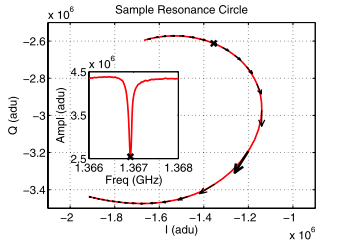
\includegraphics[clip,angle=0,width=\columnwidth]{Figures/resonance-circle.png}
  \caption{Trajectory of $\I$ and $\Q$ during a frequency sweep around the
    resonance of a KID. The arrows represent $(\di,
    \dq)$. \citep{2013A&A...551L..12C}}
  \label{circle-iq}
\end{figure}

The excitation tone frequency of a KID is modulated by a local oscillator with a
known frequency shift. This provides two values $f_{\pm} = f_0 \pm \delta
  f_{LO}/2$ with $\delta f_{LO} \simeq 1$\,kHz. The ``In-phase'' in
``in-Quadrature'' amplitudes $i(t)$ and $q(t)$ then read:

\begin{equation}
(i(t), q(t)) = (\frac{i(f_{+}) +
    i(f_{-})}{2},
\frac{q(f_{+}) + qf_{-})}{2}),
\end{equation}

and the differential values are :

\begin{equation}
\label{gradient}
(\di(t), \dq(t)) =
\left(\frac{i(f_{+}) - i(f_{-})}{\delta f_{LO}},
\frac{q(f_{+}) - q(f_{-})}{\delta f_{LO}}\right).
\end{equation}

These quantities are represented on Fig. \ref{circle-iq}. In this paper, we take
typical laboratory values and assume that $i$ and $q$ are sampled at
880\,Hz. This high acquisition rate is allowed by the sub-millisecond time
constant of the KIDs. For most experiments, such a high sampling rate is not
required and we average these measures over 40~samples to produce
four secondary quantities at 22\,Hz:

\begin{eqnarray}
\I  &=& \sum^{N_{m}=40}_{p=1} i_{p},\\
\Q  &=& \sum^{N_{m}=40}_{p=1} q_{p},\\
d\I &=& \sum^{N_{m}/2=20}_{p=1} i_{2p} - i_{2p-1},\\
d\Q &=& \sum^{N_{m}/2=20}_{p=1} q_{2p} - q_{2p-1}.
\end{eqnarray}

With these quantities in hand we have several ways to derive the transmitted
signal. They are presented in the following paragraph.

\subsubsection{\rf}
If a variation $\Delta\I(t)$, $\Delta\Q(t)$ is observed between successive ($\I$,
$\Q$) points, it is possible to estimate the shift of the resonant frequency
$\Delta f_{0}$ between these two samples by comparing ($\Delta \I$, $\Delta \Q$)
with the gradient $(\di,\dq)$ induced by the known $\delta
f_{0}$ of the local oscillator. This is done by a scalar projection of ($\Delta\I$,
$\Delta\Q$) on $(\di,\dq)$ that is tangent to the resonance circle. To have a
cleaner estimation of the latter, we take its running average over 50
points that we write $\langle . \rangle_{50}$ \citep{2014A&A...569A...9C}:

\begin{equation}
\label{eq:Rf}
\Delta f_{0} = \delta f_{LO} \frac{\Delta \I\, \langle \di
  \rangle_{50}
+ \Delta \Q\, \langle \dq \rangle_{50}}{\langle \di
  \rangle_{50}^{2}
 + \langle \dq \rangle_{50}^{2}},
\end{equation}

Note that this average is performed only on the tangent vector $(\di,\dq)$ so
that $\Delta f_0$ is sampled like $\I$ and $\Q$ at 22\,Hz. This method has been
successfully used in \todo{XXXX}, but can be affected by some systematic
uncertainty and be a source of non-linearity. Indeed, $(\di,\dq)$ is tangent to
the $(\I,\Q)$ circle for a fixed background optical power, while, in principle,
the incident optical power that induces the observable $(\Delta \I, \Delta \Q)$
should distort the resonance circle to some extent. As a consequence, the
observed $(\I,\Q)$ trajectory is not precisely parallel to the $(\di,\dq)$
direction. Early laboratory and on-site tests have shown that this approximaton
leads to a reconstruction of point source fluxes better than 2\%
\citep{2013A&A...551L..12C}. In this work, we improve this upper limit on
simulations and assess the impact of this error on futures CMB polarization
measurements.

\subsubsection{Circle fit : Cf}

\begin{figure}
\includegraphics[clip, angle=0, width=\columnwidth]{Figures/circle_zres.eps}
\caption{Bottom: location of $\I$ and $\Q$ when a KID observes a point source of
  various fluxes. Top: ratio of the distance between $(\I,\Q)$ and the center of
  the fitted circle over the radius of this circle. All the points on the pure
  imaginary line at $\I=1$ are the result of the transformation of the circle
  into $Z_{res}$ according to eqs.~(\ref{eq:z_res}) and
  (\ref{eq:scale_rotate}).}
\label{fig:circle_zres}
\end{figure}

\todo{ref to the circular nature of (I,Q): \cite{2011ApJS..194...24M}}.\\

To improve \rf, we developed a new technique that fully exploits the circular
nature of the $(\I,\Q)$ trajectory, hereafter called \cf. It is
  based on the transformation property of a circle in the complex plane into a
  straight line. Indeed, let us consider a circle centered on $(0,1/2)$ with a
  radius $1/2$ and compute its inverse:

\begin{eqnarray}
Z_{ref} &\equiv&\frac{1}{2} + \frac{1}{2}e^{i\phi}\,, \\
&=&\cos\frac{\phi}{2}e^{i\phi/2}\,,\\
Z_{res} &\equiv& 1/Z_{ref}\,, \label{eq:z_res} \\
&=&1-i\tan\frac{\phi}{2}\,.
\label{eq:z_res}
\end{eqnarray}

$Z_{res}$ is a straight line and along this line $Z$ varies linearly with
$\phi$ for small values of $\phi$. Experimentally, we are in this regime
when the signal is weak and when $\phi$ is defined w.r.t.~ the $(O,C)$ axis
as defined on Fig.~\ref{fig:circle_zres}. We thus fit the radius $r$ and the
center $(\I_c,\Q_c)$ of our measurement circle $Z=\I+j\Q$. Defining
$\alpha=\arctan\Q_c/\I_c$, we scale, rotate and translate this
circle to the $Z_{res}$ circle according to

\begin{equation}
Z_{ref} = \left(\begin{array}{c}
\I_{ref}\\
\Q_{ref}\end{array}\right) = 
\frac{-1}{2r}\left(\begin{array}{rr}
\cos\alpha & \sin\alpha\\
-\sin\alpha & \cos\alpha\end{array}\right)
\left(\begin{array}{c}
\I-\I_c\\
\Q-\Q_c\end{array}\right) +
\left(\begin{array}{c}
1/2\\
0\end{array}\right)
\label{eq:scale_rotate}
\end{equation}

The result of this transformation is shown on Fig.~\ref{fig:circle_zres}. A
variation of the signal $(\Delta\I,\Delta\Q)$ leads to a variation
$\Delta\phi$ along $Z$ that is proportional to the frequency shift $\Delta f$
that we are after to determine photometry. To derive the calibration between
these two quantities, we once again rely on the $(\di,\dq)$ that is induced by
the known $\delta f_{LO}$. Applying transformation (\ref{eq:scale_rotate}) to
$(\di,\dq)$, we obtain the corresponding variation $dy = Im(dZ_{res})$. The
final derivation of $\Delta f$ corresponding to $(\Delta\I,\Delta\Q)$ requires
the integration of $dy/\delta f_{LO}$. For the sake of simplicity, we fit
$Im(dZ_{res})$ as a polynomial of $dy/\delta f_{LO}$ that is therefore trivial
to integrate.

%% \begin{equation}
%% \tan\frac{\delta\phi}{2} \simeq \frac{\delta\phi}{2} +
%% \frac{(\delta\phi)^3}{15}
%% \end{equation}

{\color{blue} 
\subsection{Non linearity characterization with simulations}

\begin{figure}
\center
\includegraphics[clip, angle=0, width=\columnwidth]{Figures/KID-linearity-Monfardini2014.png}
\caption{KID linearity demonstrated in laboratory under realistic
  conditions. The plot shows the frequency shift of the resonance as a function
  of the optical background temperature (K). Solid line : linear fit of the
  experimental points. Credits : \citet{2014JLTP..176..787M}.}
\label{fig:KID-lin}
\end{figure}

Laboratory measurements with \todo{XXXX describe set up XXX} have shown that
KIDs are linear over a wide range of backgrounds
(Fig.~\ref{fig:KID-lin}). However, for these measurements, $\Delta f$ was not
reconstructed as described in the previous section, and we want to characterize
our formalism up to $\epsilon$ of the order of $10^{-5}-10^{-6}$. We simulate
the measure of point source by a KID and show how linear this measure remains in
various contexts. Non linearity could appear when the source is very bright
(such as planets of several tens of Jy) and the density of charge carriers is
altered. This leads to $(\I,\Q)$ meaures that leave the resonance circle, hence
invalidating the approximations made in the photometric equations of the
previous section. A second possible source of non linearity is the instrument
scanning speed. Indeed, even if the source is moderately bright, if it is
scanned too fast, $(\Delta\I,\Delta\Q)$ could be far from the tangent vector
$(\di,\dq)$ which would alter their linear relation. In this paragraph, we
explore both cases. We simulate the observation of a point source with a flux
that we vary between \todo{1 and 500\,Jy TBC}. We assume that our instrument has
a 11\,arcsec FWHM Gaussian beam like the polarized 1\,mm channel of \nikad. We
also vary the scanning speed of our virtual instrument while keeping a minimum
of 3~samples per FWHM to respect the Nyquist criterion.

Modulation of the polarization by a rotating Half Wave Plate (HWP) like in
\nika\ and \nikad\ creates a background modulation equivalent to several tens to
hundreds of Jy at frequencies close to the HWP rotation harmonics
\citep{2017A&A...599A..34R}. After early tests by \todo{cite Hildebrand in the
  80's or so ?}, this kind of modulating device has been left aside for
\todo{20~TBC} years in the context of millimetric observations. With the
improvement of technologies it progressively came back in the landscape, in
particular with pioneering experiments like \emph{Maxipol}
\citep{2007ApJ...665...42J} and \emph{EBEX} \citep{2010SPIE.7741E..1CR}. It is
now more and more common and is considered as the leading option for future
satellite designs such as \emph{LiteBIRD} \todo{add ref}. Such a background must
be accounted for in the simulations.






%% In the context of a CMB experiment mapping a large fraction of the sky, one
%% should also consider the CMB dipole with its 6.73\,mK peak to peak \todo{ADD
%%   REF} converts into a \todo{XXX\,Jy} signal \todo{Account for the bandpass
%%   !!}. It can displace the zero level $Z$ along the circle so that a
%% bright source would enter the non linear regime sooner than expected. This is
%% also true for strong Galactic emission like that of Dust at frequencies above
%% $\sim 100$\,GHz. It is even truer for the background modulation induced by a
%% rotating Half Wave Plate (HWP). After early tests by \todo{cite Hildebrand in
%%   the 80's or so ?}, this kind of modulating device has been left aside for
%% \todo{20~TBC} years in the context of millimetric observations. With the
%% improvement of technologies, it progressively came back in the landscape, in
%% particular with pioneering experiments like \emph{Maxipol}
%% \citep{2007ApJ...665...42J} and \emph{EBEX} \citep{2010SPIE.7741E..1CR}. It is
%% now more and more common and is considered as the leading option for future
%% satellite designs such as \emph{LiteBIRD} \todo{add ref.}. \nika\ has used a
%% fast and continously rotating HWP and saw strong parasitic signal synchronous
%% with the HWP rotation harmonics \citep{2017A&A...599A..34R} like \emph{Maxipol}
%% and \emph{EBEX} (cf.~Fig.~\ref{fig:hwp_power_spectrum}). The amplitude of this
%% signal is comparable to bright planets at several tens of Jy and could also bias
%% the average position of the $Z$ measurement and hence the photometry.

}







%%  The idea of this
%% method is to project $\I$, $\Q$, $d\I$, $d\Q$, onto an axis $y'$ which is
%% as linear as possible with frequency and thus with the incident optical
%% power. Let's denote $Z = \I + j\Q$, near the resonance circle we have:
%% 
%% \begin{equation}
%% f - f_{0}= \frac{w}{2} \tan \frac{\phi}{2}.
%% \label{eq:hyp-f}
%% \end{equation}
%% 
%% \todo{what are $w$ and $\phi$?}\\
%% The idea is to construct $y'$ from a circle $Z$. The inverse of $Z$ is a circle
%% but we can normalize it to transform it into an infinite radius circle that is
%% expected to be linear with the KID frequency.  To do so we define a reference
%% circle which is centered on ($\frac{1}{2},0$) and has a radius of $\frac{1}{2}$,
%% after using trigonometric relations we obtain :
%% 
%% \begin{equation}
%% Z_{ref} = \cos \frac{\phi}{2} e^{j \phi/2}.
%% \label{eq:Zref}
%% \end{equation}
%% 
%% If we inverse Eq.~(\ref{eq:Zref}), we have : 
%% \begin{equation}
%% Z_{res} = 1 - j \tan \frac{\phi}{2}.
%% \label{eq:Zres}
%% \end{equation}
%% 
%% The imaginary part of Eq.~(\ref{eq:Zres}) is linearly dependant on the frequency
%% defined in Eq.~(\ref{eq:hyp-f}), and represents the new axis $y'$.
%% 
%% From the KID model we have $Z=\I+j\Q$. We do a series of transformations on this
%% circle to make it identical to the reference circle, the final result is named
%% $Z'$, with $Z'=p[ZM_{r} + T]$. p is the scaling factor, T represents the
%% translation and $M_{r}$ is the rotation matrix :
%% 
%% \begin{equation}
%% M_{r} = 
%% \begin{pmatrix}
%% 	\cos \alpha & \sin \alpha \\
%% 	-\sin \alpha & \cos \alpha
%% \end{pmatrix} .
%% \end{equation}
%% 
%% 
%% First we rotate $Z$ :
%% \begin{equation}
%% Z' = 
%% \begin{pmatrix}
%% 	\cos \alpha & \sin \alpha \\
%% 	-\sin \alpha & \cos \alpha
%% \end{pmatrix}
%% \begin{pmatrix}
%% 	\I\\
%% 	\Q
%% \end{pmatrix}
%% =
%% \begin{pmatrix}
%% 	\I\cos \alpha + \Q\sin \alpha\\
%%   - \I\sin \alpha + \Q\cos \alpha
%% \end{pmatrix}.
%% \end{equation}
%% 
%% Then we translate and rescale it, to obtain $Z'=\I'+j\Q'$ with : 
%% \begin{eqnarray}
%% \I' &=& \frac{1}{2r}[(\I-x_{c}) \cos \alpha + (\Q - y_{c}) \sin \alpha] + \frac{1}{2}, \\
%% \Q' &=& \frac{1}{2r}[-(\I-x_{c}) \sin \alpha + (\Q - y_{c}) \cos \alpha]. \\
%% \end{eqnarray}
%% 
%% ($x_{c}, y_{c}$), r and $\alpha$ respectively, the center, radius and rotation
%% angle of the initial circle. The derivative of the inverse of $Z'$ is
%% $dZ_{res}=-dZ'/Z'^{2}$, with :
%% 
%% \begin{eqnarray}
%% dZ' &=& d\I' + jd\Q',\\
%% d\I' &=& -\frac{1}{2r}(d\I \cos \alpha + d\Q \sin \alpha), \\
%% d\Q' &=& \frac{1}{2r}(-d\I \sin \alpha + d\Q \cos \alpha).
%% \end{eqnarray}
%% 
%% The imaginary part of $Z_{res}$ and $dZ_{res}$ represent respectively $y'$ and
%% $dy'$ which are proportional to the KID frequency. We can use these quantities
%% to calibrate $y'$ and derive the frequency of the KID. In fact, according to the
%% hypothesis in Eq.~(\ref{eq:hyp-f}), $f$ is a polynomial, so to reconstruct the
%% shift of the resonant frequency we can fit $\frac{\Delta f}{dy_{3}} = R_{n}(y')$
%% by a polynomial function, where $R_{n}$ is a polynomial function with a degree
%% $n$. It is then easy to integrate $R_{n}$ into $P_{n+1}$, with
%% $\overset{.}{P_{n+1}}=R_{n}$ to obtain the relative frequency of the KID :
%% 
%% \begin{equation}
%% f - f_{0} = P_{n+1}(y')
%% \end{equation}
%% 
%% \todo{keep for global conclusion:} In conclusion, because we can not directly
%% measure the optical power from a KID, new methods were developed to monitor the
%% shift of the resononance frequency of the detector. First with the modulated
%% readout technique we can calculate four quantities : $\I$, $\Q$, $\di$,
%% $\dq$. With these quantities in hand, we can monitor the shift of the resonant
%% frequency and derive the corresponding incident power ny using the two methods
%% that were developed : \rf\ which is already successfully used in \nika\ and
%% \nika2\ (see \citep{2014A&A...569A...9C}) , and \cf\ which is an improvement
%% from \rf . In this paper, we compare these two methods in terms of linearity. To
%% do so, in the next sections we do simulations of observations by a KID and we
%% use \rf\ and \cf\ to reconstruct the signal. We then study the impact of the KID
%% non-linearity on the search for B modes polarization of the CMB.

%\section{Application to CMB maps and power spectra estimations}
\section{Non linearity and impact on CMB polarization measurements}
\label{sec:cmb}

Detecting CMB polarization $B$ modes is one of the major challenges in modern
cosmology. However, due to the faintness of the expected signal, systematic
effects must be controlled to challenging low levels. The specific way KID
photometry is derived is as new as this technology and we here investigate if it
might lead to non linearty in the photometry reconstruction, and how this would
impact CMB polarization measurements.

\subsection{Parameterization}

We assume that KIDs are placed right after a perfect polarizer along the optical
path. At each time, they therefore measure a combination of the Stokes
parameters $I$, $Q$ and $U$. To first order, the non linearity of the KID
response can be described by a parameter $\epsilon$ such as:

\begin{eqnarray}
m &=& \phi + \epsilon\phi^2 \nonumber \\
&=& (I+Q\cos2\alpha+U\sin2\alpha) + \epsilon(I+Q\cos2\alpha+U\sin2\alpha)^2 \nonumber\\
 &\simeq & (I + \epsilon I^{2}) + (Q + 2\epsilon IQ) \cos(2\alpha) + (U + 2 \epsilon IU) \sin(2\alpha)
\label{eq:eq-NL}
\end{eqnarray}

The non-linearity coefficient depends on the detector response. In fact, it is a systematic effect of the instrument and as a consequence will always impact our measurements. This non-linearity can lead to leakage of the CMB and dust temperature signal into the polarization maps and consequently can induce spurious polarization signals which could prevent us from detecting $B$ mode polarization. \eps\ is constituted of several components such as \eps\ related to the CMB and dust. $T_{dust}$ has more effect on the leakage than $T_{CMB}$  that is why we will focus on dust.
To study this effect we simulate spurious signals from a map of the galaxy (dust) observed by Planck (REF) by applying the non-linear mapping described by Eq.~(\ref{eq:eq-NL}) :

\begin{eqnarray}
\label{eq:spurious-mapI}
\Delta I_{dust}  &=& \epsilon I_{dust}^{2},\\
\label{eq:spurious-mapQ}
\Delta Q_{dust}  &=& 2\epsilon I_{dust}Q_{dust},\\
\label{eq:spurious-mapU}
\Delta U_{dust} &=& 2 \epsilon I_{dust}U_{dust}.
\end{eqnarray}

To investigate the different modes of CMB polarization we used the HEALPix package \citep{2005ApJ...622..759G} to generate modified power spectra from the spurious polarization maps. They are described by Eq.~(\ref{eq:eq-cl}) and are represented in Fig.~\ref{fig:cl2}.

\begin{equation}
\Delta C_{l} = \epsilon'^{2} C_{l}^{XX'},
\label{eq:eq-cl}
\end{equation}
Where $\lbrace X,X' \rbrace$ = $\lbrace T,E,B \rbrace$ .\\

\begin{figure}[h]
\center
	\includegraphics[clip, angle=0, width=\columnwidth]{Figures/cl2_spurious.eps}
	\caption{Power spectra for spurious temperature and polarization anisotropies. The black, blue and red curves indicate the $EE$, $TE$ and $BB$ power spectra. The bottom three red curves represents the $BB$ power spectra for a tensor-to-scalar ratio r = (T/S) = 0.1, 0.01, 0.001.}
	\label{fig:cl2}
\end{figure}

Here we will focus on the leading spurious term $C_{l}^{TE}$ : 
\begin{equation}
\Delta C_{l}^{BB} = \epsilon^{2} C_{l}^{TE}.
\label{eq:eq-cl2}
\end{equation}

The leakage of temperature into polarization is represented by the coefficient \eps\ of Eq.~(\ref{eq:eq-cl2}). To determine this coefficient, we compute :

\begin{equation}
\epsilon = \sqrt{\dfrac{r/10}{C_{l}^{TE}}},
\label{eq:eq-cl3}
\end{equation}

they are represented in Tab. \ref{tab:eps-lkg}

\begin{table}[h!]
\center
	\begin{tabular}{|c|c|c|c|}
  	\hline
 	\backslashbox{$\epsilon$}{$r$} & 0.1 & 0.01 & 0.001 \\
	\hline
	$\epsilon'$ & 7.90 x $10^{-4}$ & 2.50 x $10^{-4}$ & 7.90 x $10^{-5}$\\
  	\hline
	\end{tabular} 
\caption{Non-linear coefficients related to the leakage of temperature into polarization for scalar-to-tensor ratio r = (T/S) = 0.1, 0.01, 0.001.}
\label{tab:eps-lkg}
\end{table}

In the search of $B$ modes polarization, Planck anticipated a $r$ detection threshold of 0.1 . In Tab. \ref{tab:eps-lkg}, we calculated \eps\ for lower tensor-to-scalar ratio ($(T/S) = 0.1, 0.01, 0.001$). To be able to detect $B$ modes polarization at this level without being contaminated by the leakage of temperature into polarization, the non-linearity coefficient related to the detector and the signal reconstruction must be lower than \eps\ of Eq.~(\ref{eq:eq-cl2}). By satisfying this criteria we can satisfy the other \eps\ from Eq.~(\ref{eq:eq-NL}) because $C_{l}^{TE}$ from dust temperature is the leading spurious term. 

To conclude, the study of CMB polarization and the measurement of $B$ modes polarization represent one of the major challenges in modern cosmology. The detection of $B$ modes can be affected by a leakage effect of temperature into polarization. Here we studied the non-linearities that the leakage from dust temperature can create. We have seen that the non-linearity coefficients are ranged between $10^{-4}$ and $10^{-5}$.\\

To search for $B$ modes at low tensor-to-scalar ratio, the non-linear coefficient of the detector that we use has to be lower than \eps . In the next section, we will study a systematic effect of KIDs by calculating their non-linearity coefficient, and comparing them to \eps .


\section{KIDs specific systematics and application to CMB polarization}

\begin{itemize}
\item glitch (because it's important in a space oriented discussion)
\item non linearity. Explain frequency modulation, RF and PF reconstructions
  that may not be strictly linear
\item Explain what we mean by non linearity (ref to previous papers that showed
  the linearity of the KIDs response and that we look at the next order
  correction). Polarized equations with the non linear term.
\item Describe the simulation method : on simule une planete scannee a une
  certaine vitesse, on recalcule le flux etc... pour mesurer la
  non-lin\'earit\'e.
\item Results in RF and PF
\item Application to CMB maps and power spectra estimation
\item HWP associated systematics. The modulation of the HWPSS may bias the
  measurement by inducing non linearity.
\end{itemize}

In view of future utilizations of KIDs in space mission it is necessary to demonstrate the capabilities and the suitability of KIDs arrays in a space like environment. In this section we will adress some of the systematics effects that need to be taken into account during the design of futur generation detector arrays for space applications, such as the KIDs non-linearity.\\

\subsection{Cosmic rays impact on KIDs array}

One of the major problems for space based missions is the impact of an intense flux of high energy particles, referred to as Cosmic Rays (CR) on the detectors. Primary CR are produced by the Sun and by other galactic sources. They are mostly composed by protons (90\%), helium nuclei (9\%) and a few heavier nuclei and electrons (1\%). The CR spectrum is peaked aroud 200 MeV, thus the particles have sufficient energy to penetrate the detectors and give an unwanted signal. The Planck satellite \citep{2014A&A...571A..10P} has demonstrated that the impact of CR on the detectors are a key problem for space missions. Indeed, the glitches caused by CR can mask the real data and induce a loss of an important fraction of it.\\
Experiments have been done to construct a setup that allows to study the behavior of KIDs arrays under typical conditions of a space-borne observatory, and establish the compatibility of KIDs with a space environment \citep{2016A&A...592A..26C,2016SPIE.9914E..0NM}. When the detector is hit by a CR there is a lapse of time during which the sensor is 'blind' to the incoming scientific data. The length of this dead-time depends on the response time of the KID (time constant) which is determined by the quasi particle lifetime. \citet{2012ApPhL.100w2601M} have shown for KID, this time constant is equal to about tens of microseconds which is faster than bolometers (from 5-10 ms to 2s). This means that for the same CR hit, less data is lost when using KIDs arrays. Plus, the experiments have confirmed the fact that KID recover their initial state in less than 5 milliseconds. Finally, \citet{2016SPIE.9914E..0NM} concluded that the percent level of data loss per pixel by a KIDs array placed in a space environment is about 1 \% compared to 15 \% for Planck HFI bolometers.\\ Compared to bolometers, the KID technology shows promising results for compatibility with a space-borne mission, as their extremely short glitch time constant permits to greatly reduce the data loss fraction due to CR impacts. 

\subsection{KIDs non-linearity}

One of the key systematic effect that we must take into account is the KID non-linearity induced by the detector and the method we use to reconstruct the absorbed signal. In this paper, we will focus on the KID non linearity and how it impacts on a measurement of the CMB polarization.\\

The KIDs linearity has been demonstrated, over a large power range, in laboratory under realistic conditions as shown in Fig. \ref{KID-lin}. As we can see, at 300K the response of the KID is still under a linear regime.

\begin{figure}[h]
\center
	\includegraphics[scale=0.4]{KID-linearity-Monfardini2014.png}
	\caption{KID linarity demonstrated in laboratory under realistic conditions. Y-axis : frequency shift of the resonance (KID measured signal), X-axis : optical background temperature. The solid line represents the linear fit of the experimental points. Credits : \citet{2014JLTP..176..787M}.}
	\label{KID-lin}
\end{figure}

In this section we look at the next order correction, meaning that we will focus on the non-linear term produced by the detector and the way that we reconstruct the signal. A measure done by the KID is defined by $m = T + P$, with $T$ and $P$ representing the temperature and polarization. The non-linearity is characterized  by the $\varepsilon$ coefficient in $ m = m_{1} + \varepsilon m_{1}^{2}$. We have : 

\begin{equation}
\begin{split}
m & = m_{1} +\varepsilon' (T+P)^{2} \\
 & = T + P + \varepsilon'(T^{2} + P^{2} + 2TP) 
\end{split}
\end{equation}

Therefore, knowing that $T=I$ and $P = Q\cos(2\alpha) + U \sin(2\alpha)$, the polarized equation with a non-linear term is given Eq. \ref{eq-NL}.

\begin{equation}
m  \simeq (I + \varepsilon' I^{2}) + (Q + 2\varepsilon' IQ) \cos(2\alpha) + (U + 2 \varepsilon' IU) \sin(2\alpha)
\label{eq-NL}
\end{equation}

The non-linear coefficient $\varepsilon'$ is induced by the detector and the method used to reconstruct the signal.

\subsection{Application to CMB maps and power spectra estimations}
The measurment of CMB polarization, and especially the detection of B modes, is one of the major challenges in modern cosmology. In this paper, we show that the KIDs systematic effect such as the non-linearity does not affect them from detecting B modes.

The non-linearity coefficient $\varepsilon'$ does not intervene in the pointing strategy, in fact it is a systematic effect of the instrument and as a consequence will always impact our measurments. \\
To take into account this effect we simulate CMB maps with a PLANCK pointing strategy (citer ref) which follows Eq. \ref{eq-NL}, by using HEALPIX (citer ref).
Eq. \ref{eq-NL} is translated in the the power spectrum by Eq. \ref{eq-Cl}.

\begin{equation}
C_{l}^{s} \propto p^{2} \varepsilon^{2} C_{l}
\label{eq-Cl}
\end{equation}
Where $C_{l}^{s}$ is the systematic power spectra.\\

We generate I, Q, U maps from observed $C_{l}$ to which we apply the non-linear mapping described by Eq.\ref{eq-NL}. This will produce spurious polarization signals from which we can derive modified $C_{l}^{s}$ and $\varepsilon$ represented in Eq. \ref{eq-Cl}. We found 

\begin{equation}
\varepsilon^{2} \simeq 4.10^{-7}
\label{epsilon}
\end{equation}

This non-linearity can lead to leakage of the CMB temperature signal into the polarization maps and consequently can induce spurious polarization signals which could prevent us from detecting B mode polarization. The leakage effect is represented by the coefficient $\varepsilon$ of Eq. \ref{eq-Cl}. As a result, to be able to detect B mode polarization, the non-linearity coefficient related to the signal reconstruction must be lower than $\varepsilon^{2} \simeq 4.10^{-7}$.

%To do so, we calculate the non-linearity coefficient $\varepsilon'$ given by Eq.\ref{eq-NL} with a tolerance on mode B contamination by generating I, Q, U maps from observed $C_{l}$. Then we apply the non linear mapping described by Eq.\ref{eq-NL}, this will generate spurious signal from wich we derive modified $C_{l}$. 


\subsubsection{Definition d'une strategie de pointage}

\subsection{HWP associated systematics}


\section{Conclusion}
\label{conclusion}

This paper presents the study of KIDs systematic effects such as the non-linearity and an application to the CMB polarization. 
KIDs are a new kind of detectors based on superconducting technology that provides high sensitivity. They have been developed for the construction of NIKA and NIKA2 since 2007, which is now the first operational instrument using KIDs. One of the key asset of KIDs is their natural multiplexing capability which makes them one of the best candidates for future space mission that needs large size detector array. In this context, in a first part, we studied the response of a KID by using two methods to reconstruct the signal (\rf and \cf) and its systematic effects caracterized by its non-linearity coefficient \eps. For an incoming source consisting of a planet of 500 Jy, the dipole and a HWP, and for different scan speed, we found $\varepsilon_{rf}$ $\simeq 10^{-5}$ and $\varepsilon_{cf}$ $\simeq 10^{-7}$. The non-linearity depends on the way that we reconstruct the signal, and even if \rf can reconstruct the signal very well, \cf is better at it and generates less non-linearities. Another good point is that the modulation of the HWP does not bias the measurement by inducing large non-linearities. We have seen that in order to have less non-linearities, we need to put constraints on the scanning speed, so in a second part, we did more realistic simulations, by scanning a map of the Galaxy and dipole by using satellite pointing strategies. We found, that depending on the incoming sources, $\varepsilon_{rf}$ varies between $10^{-7}$ (Galaxy only) and $10^{-3}$ (Galaxy, dipole, HWP), and $\varepsilon_{cf}$ varies between $10^{-8}$ (Galaxy only) and $10^{-4}$ (Galaxy, dipole, HWP) (POLSAT, VOIR PB PLANCK). The results show that in a space context KIDs are capable of accurately reproducing the signal and that as in the precedent simulations \cf is slightly better than \rf.\\
The measure of CMB $B$ modes polarization is a major goal of observational cosmology, as their detection would sign the presence of primordial gravitational waves and provide a confirmation of inflation. Observations of CMB polarization demand a high control of systematics effect and in light of this, we demonstrated the capabilities of KIDs arrays to detect B modes polarization by comparing systematic effects coming from the detector and the leakage of dust temperature into polarization maps. With HEALPix, we simulated spurious signals from a map of the Galaxy and generated modified $C_{l}$. From $C_{l}^{TE}$, we calculated the coefficient ($\varepsilon'$) related to the leakage of temperature into polarization. For a tensor-to-scalar ratio (T/S) = 0.1, 0.01, 0.001 we respectively found $\varepsilon' \simeq 2.51$x$10^{-2}$, 7.95x$10^{-3}$, 2.51x$10^{-3}$. Because the leakage of temperature into polarization maps is the systematic effect that is most likely to contaminate the detection of $B$ modes , to be able to measure them, the non-linear coefficient $\varepsilon$ related to the detector must be lower than $\varepsilon'$. In all of the precedent simulations, $\varepsilon $ varried between $10^{-3}$ and $10^{-8}$, so $\varepsilon < \varepsilon'$, therefore we can say that the KID is capable of detecting $B$ mode polarization. Finally, because of the KID multiplexing ability and its capability of detecting $B$ mode polarization, we can say that KID technology is developping toward becoming one of the best candidates to space mission and study of the CMB polarization.
 
\bibliography{biblio}

%-----------------------------------------------------
\begin{acknowledgements}
NIKA standard acknowledgements + FOCUS + E.~Hivon.
\end{acknowledgements}

\end{document}
